Since Deep Convolutional Neural Networks (CNNs) became the most powerful algorithm in object recognition task, fine-tuning the deep CNNs has become a popular and effective way to transfer the knowledge between different visual recognition tasks. The intuition of fine-tuning the deep CNNs for transfer learning is that low-level features, such as edges and lines, are universal for object recognition while high-level features, which are the combinations of the low-level features, are more specific for the designed task. Because deep CNNs can learn hierarchical features, from abstract low-level features to detailed high-level ones, by changing the combinations of the low-level features in the pre-trained deep CNNs, the high-level features can be learned effectively for the new recognition task \cite{farabet2013learning}.

\begin{figure}
	\centering
	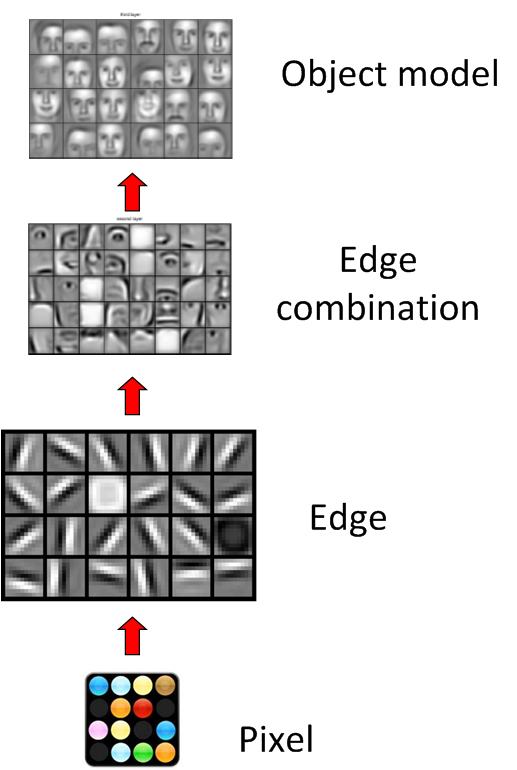
\includegraphics[scale=.7]{relatedwork/fig/hierachy}
	\caption{Hierarchical Features of Deep Convolutional Neural Networks for face recognition.}
\end{figure}

Applying the pre-trained model from ImageNet dataset on other object recognition benchmark datasets shows some impressive results. Zeiler et al.  \cite{zeiler2014visualizing} applied their pre-trained model on Caltech-256 with just 15 instances per class and improved the previous state-of-the-art in which about 60 instances were used, by almost 10\%.
Chatfield et al.  \cite{Chatfield14} used their pre-trained model on the VOC2007 dataset and outperformed the previous state-of-the-art by 0.9\%.
Agrawal et al. \cite{agrawal2014analyzing} show that even in the mid-level features, there are some grandmother cells, which can capture the high-level features of specific objects. Hoffman et al. \cite{hoffman2013one} show that even with one labeled example per class, it is possible to fine-tune the pre-trained deep CNNs and obtain a good classifier for some new recognition tasks. Zhou et al. \cite{NIPS2014_Zhou} provided the state-of-the-art performance using the deep features on some scene benchmarks by fine-tuning the deep CNNs. Yosinski et al. \cite{yosinski2014transferable} investigated the transferability of the layers in deep CNNs and show that the target task can be benefited from pre-training even though the source and target tasks are distant. 

In this thesis, we also use the pre-trained deep CNNs to learn new categories for food recognition and investigate the affects of each layer in deep CNNs for knowledge transfer in chapter \ref{sec:cnn}.